\chapter{Dynamical Processes in Biomedicine}
\label{cha:bio_background}

\dictum[Rosalind Franklin, \textit{Report} (1952)]{%
  The results suggest a helical structure (which must be very closely packed) containing probably 2, 3 or 4 coaxial nucleic acid chains per helical unit and having the phosphate groups near the outside.}%
\vskip 1em

...


\chapter{Optimal Transport for Dynamical Systems}
\label{cha:theory_background}

\dictum[Elinor Ostrom, \textit{Governing the Commons} (1990)]{%
  The power of a theory is exactly proportional to the diversity of situations it can explain.}%
\vskip 1em


Optimal transport theory~\citep{santambrogio2015optimal} is a central component of the machine learning toolbox and has become within a few years the go-to framework to analyze, model, and solve an ever-increasing variety of tasks involving probability measures. This is best exemplified by its increasing importance to fitting generative models, where the goal is to learn a map~\citep{arjovsky2017wasserstein, genevay2018learning, salimans2018improving}, or more generally a diffusion \citep{song2020score, de2021diffusion} to morph a simple measure (e.g., Gaussian) onto a data distribution of interest (e.g., images). This is also apparent in the many applications that use OT to align probability measures that have since arisen, e.g., to transfer label knowledge between datasets~\citep{flamary2016optimal, singh2020model}, to analyze sampling schemes~\citep{dalalyan2017theoretical}, or study population trajectories~\citep{schiebinger2019optimal, bunne2021learning}.
In this chapter, we primarily cast light on the static and dynamic formulation of optimal transport, and simultaneously establishing their theoretical nexus to provide a solid foundation for the discussion ahead.


\section{Static Optimal Transport} \label{sec:background_ot_static}

Optimal transport takes dual roles as it induces a mathematically well-characterized distance measure between distributions as well as provides a geometry-based approach to realize mappings between two probability distributions.
This section introduces the mathematical foundations of the \textbf{static} OT problem and recalls its mathematical history from \citeauthor{monge1781histoire} (\citeyear{monge1781histoire}) and \citeauthor{kantorovich1942transfer} (\citeyear{kantorovich1942transfer}) to modern Fields medal winners \citeauthor{villani2009optimal} (\citeyear{villani2009optimal}) and \citeauthor{figalli2010optimal} (\citeyear{figalli2010optimal}). 
It further provides an extended analysis of the \citeauthor{monge1781histoire} map, which provides an actionable way to flow from one probability distribution onto another, and in particular provide a complete proof of the celebrated \citeauthor{brenier1987decomposition} theorem for general costs, which will require an introduction to the notion of $c$-concavity. This quintessential result and its particularization to translation-invariant costs will lay the foundation of the flurry of neural approaches proposed in the literature and subject of this thesis. 
In particular, with respect to approaches that are a direct consequence of the \citeauthor{brenier1987decomposition} theorem, modeling Monge maps as gradients of convex functions, parameterized through convex neural networks \citep{amos2017input, huang2021convex, makkuva2020optimal, korotin2021neural, lubeck2022neural, bunne2022supervised}, via regularizers \citep{uscidda2023monge}, amortized optimization \citep{amos2022amortizing, amos2022meta}, or entropic maps \citep{pooladian2021entropic, pooladian2023minimax, divol2022optimal, cuturi2023monge}.

\begin{figure}[t]
  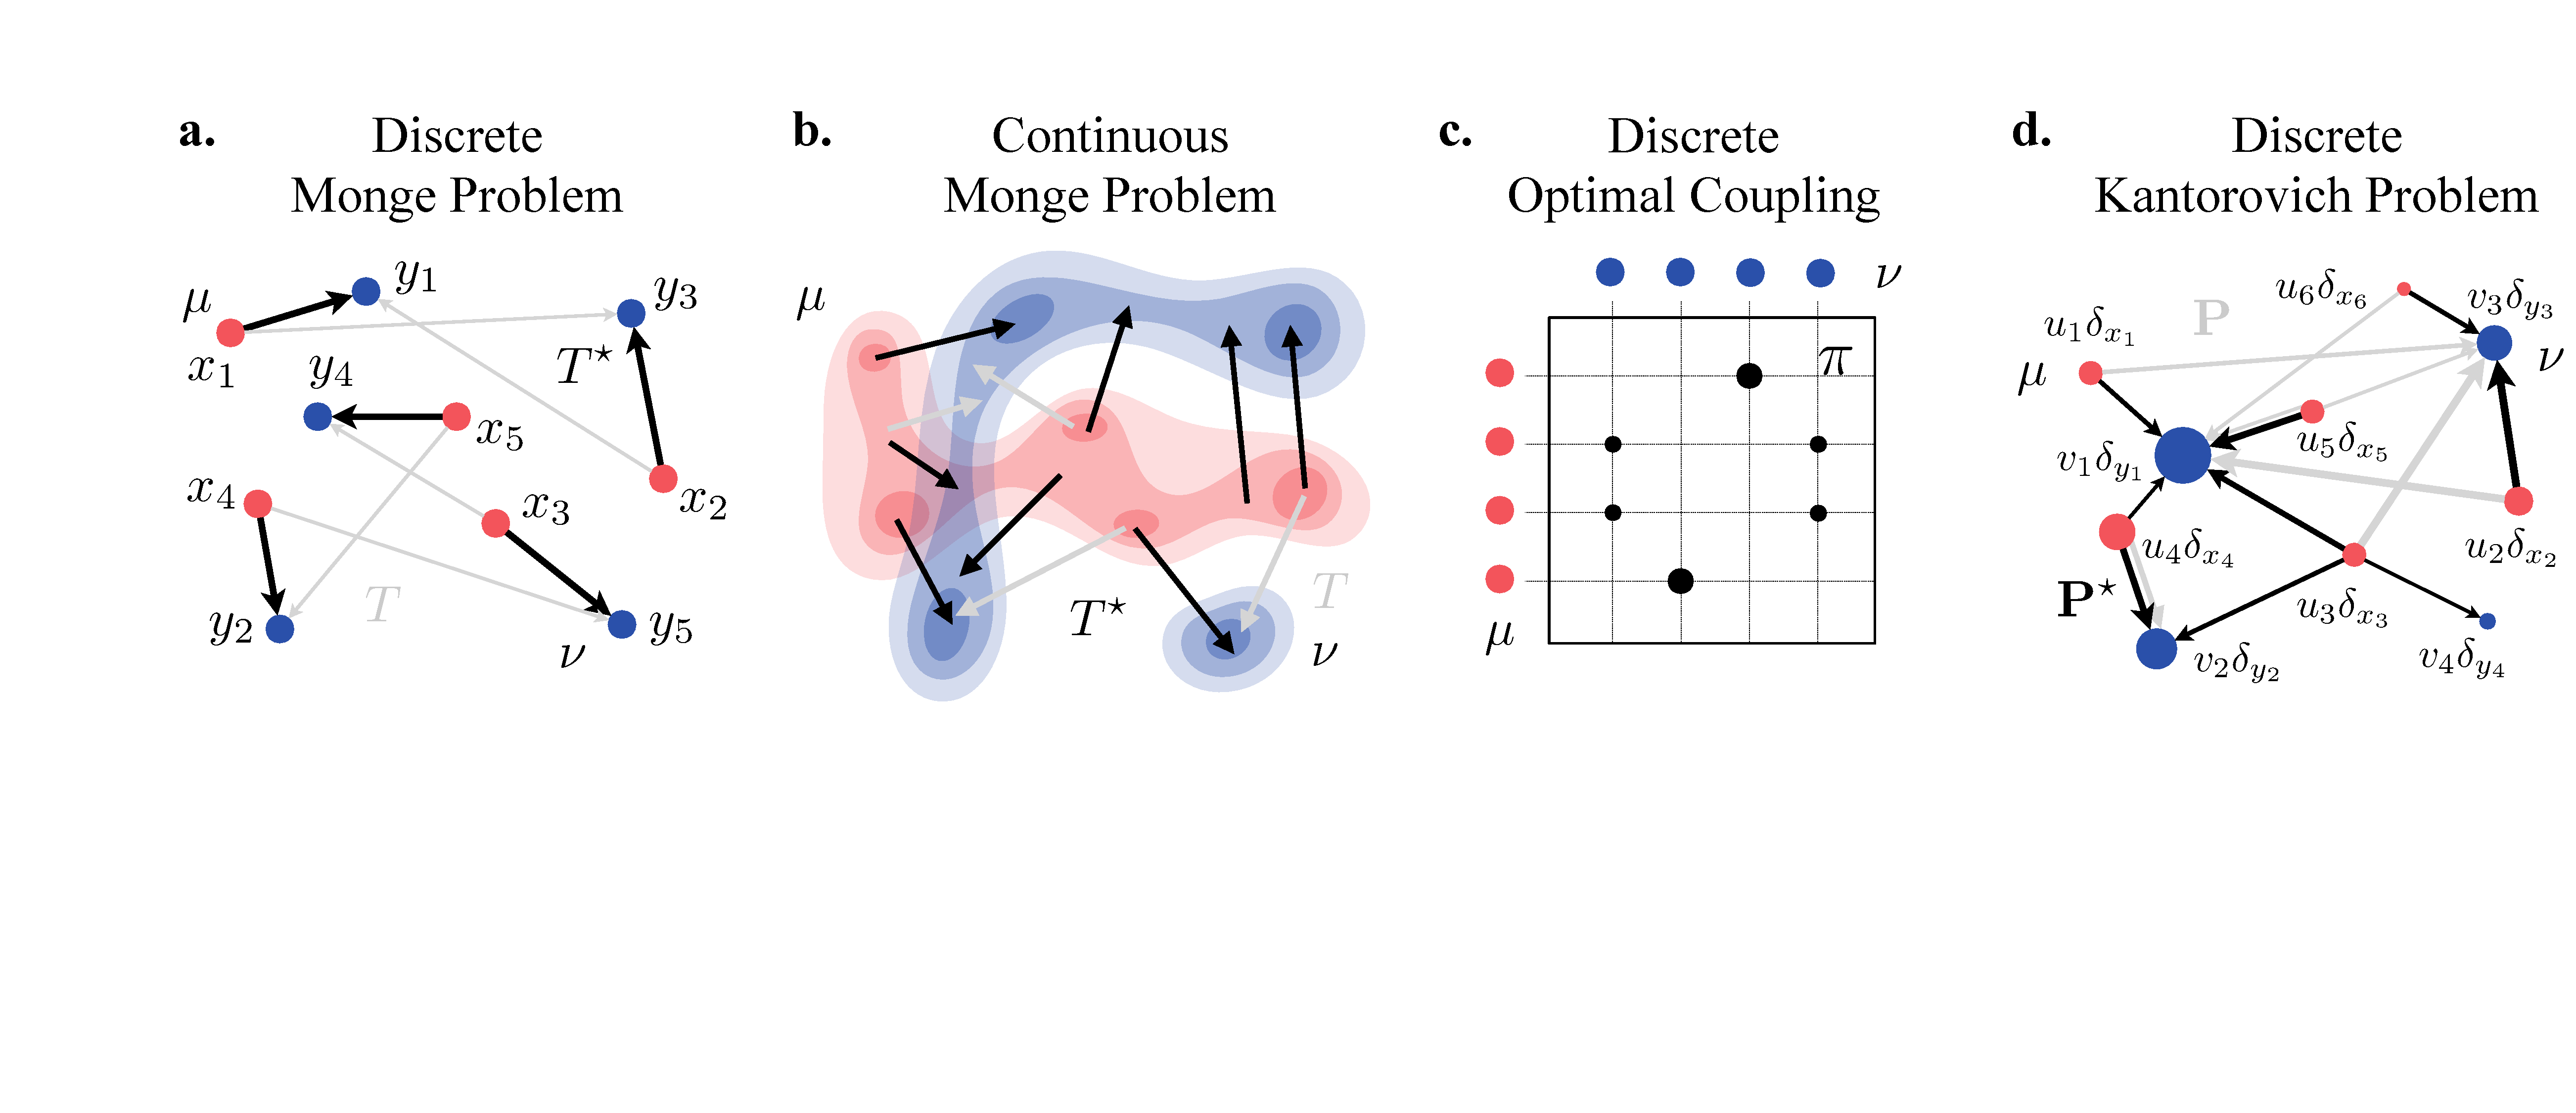
\includegraphics[width=\textwidth]{figures/fig_ot_background.pdf}
  \caption{\textbf{Overview on different formulations of the static OT problem for discrete and continuous measures.} \textbf{a.} ... \textbf{b.} ... \textbf{c.} ... \textbf{d.} .... Figure adapted from \citet{peyre2019computational}.}	
  \label{fig:ot_principles}
\end{figure}

\subsection{Monge Problem} \label{sec:background_monge}

In the 18th century "M{\'e}moire sur la th{\'e}orie des d{\'e}blais et des remblais", Gaspard Monge sets out to solve what is now known as the \citeauthor{monge1781histoire} problem; posing a seemingly simple, yet fundamentally complex question: Given two quantities of mass located at two different sites, what is the most efficient way to transport one to the other?
In more formal terms, provided with two measures $\mu, \nu\in \mathcal{P}(\mathbb{R}^d)$, here restricted to measures supported on $\mathbb{R}^d$, Monge's initial approach was to find a map $T$ that pushes one mass onto the other in a way that minimizes the total cost of transport.
Given a measurable const function $c: \mathcal{X} \times \mathcal{Y} \rightarrow \mathbb{R}$, the \citeauthor{monge1781histoire} problem then reads
\begin{equation}\label{eq:monge}
T^\star := \arg\inf_{T\sharp\mu=\nu}\int_{\mathbb{R}^d} c(x, T(x)) d\mu(x)\,.
\end{equation}
For two discrete measures $\mu=\sum_{i=1}^n u_i \delta_{x_{i}}, \nu=\sum_{j=1}^m v_j \delta_{y_{j}}$, it seeks a transport map $T: \mathcal{X} \rightarrow \mathcal{Y}$ associating each source point $x_i$ to a target point $x_j$ (see \cref{fig:ot_principles}a for the discrete and \cref{fig:ot_principles}b for the continuous setting).
The existence of $T^\star$ is guaranteed under fairly general conditions \citep[Theorem 1.22]{santambrogio2015optimal}, which require that $\mu$ and $\nu$ have finite $L_2$ norm, and that $\mu$ puts no mass on $(d-1)$ surfaces of class $\mathcal{C}_2$.


\subsection{Kantorovich Relaxation} \label{sec:background_kantorovich}

It was not until the 20th century, however, that the concept found a more tractable development. In \citeyear{kantorovich1942transfer}, Leonid \citeauthor{kantorovich1942transfer} provided a relaxation to this non-convex and difficult-to-solve problem.
Instead of the deterministic matching proposed by \citeauthor{monge1781histoire}, Kantorovich considered probabilistic correspondences that allow for transportation of mass from a single source point to various target points (mass splitting).
\begin{equation} \label{eq:kantorovich}
    W(\mu, \nu) = \inf_{\pi\in \Pi(\mu,\nu)}\iint c(x, y) \pi(dx, dy),
\end{equation}
where $\Pi(\mu, \nu)$ is the set of couplings on $\mathbb{R}^d\times\mathbb{R}^d$ with respective marginals $\mu, \nu$ (see \cref{fig:ot_principles}c). 
When instantiated on finite discrete measures, such as $\mu=\sum_{i=1}^n u_i\delta_{x_i}$ and $\nu=\sum_{j=1}^m v_j\delta_{y_j}$, this problem translates to a linear program, which can be regularized using an entropy term~\citep{cuturi2013sinkhorn,peyre2019computational}. For $\varepsilon\geq0$, set 
\begin{equation}\label{eq:reg-ot}
\We(\mu,\nu) \defeq \min_{\bP\in U(u, v)} \dotp{\bP}{[c(x_i, y_j)]_{ij}}  \,-\varepsilon H(\bP),
\end{equation}
where the discrete entropy is defined as $H(\bP) \defeq -\sum_{ij} \bP_{ij} (\log \bP_{ij} - 1)$ and the polytope $U(u, v)$ is the set of $n\times m$ matrices $\{\bP\in\mathbb{R}^{n \times m}_+, \bP\mathbf{1}_m =u, \bP^\top\mathbf{1}_n=v\}$. 
Notice that the definition above reduces to the usual Wasserstein distance when $\varepsilon=0$. Setting $\varepsilon>0$ yields a faster and differentiable proxy to approximate $W_{0}$, but introduces a bias, since $\We(\mu,\mu)\ne 0$ in general.
Regularizing objective \eqref{eq:kantorovich} with an entropy term results in significantly more efficient optimization \citep{cuturi2013sinkhorn} and differentiability w.r.t. its inputs, and thus commonly used as a loss function in machine learning applications, e.g., for structured prediction \citep{frogner2015learning,janati2020multi} or generative model fitting \citep{arjovsky2017wasserstein, salimans2018improving, genevay2018learning}.


\subsection{Kantorovich Duality} \label{sec:background_dual}

...

\subsection{Brenier's Theorem} \label{sec:background_brenier}

celebrated \citeauthor{brenier1987decomposition} theorem \citeyearpar{brenier1987decomposition}, which states that there must exist  a unique (up to the addition of a constant) potential $f^\star:\mathbb{R}^d\rightarrow \mathbb{R}$ such that $T^\star = \nabla f^\star$. 
This theorem has far-reaching implications: It is sufficient, when seeking optimal transport maps, to restrict the computational effort to seek a "good" convex potential, such that its gradient pushes $\mu$ towards $\nu$. 

This result has been exploited to propose neural OT solvers, and  will recurrently permeate this thesis, proving its essential nature in multiple instances and modern developments of optimal transport.
In practice, Monge maps can be estimated using a dual formulation~\citep{makkuva2020optimal, korotin2020wasserstein, bunne2022proximal, alvarez2021optimizing, mokrov2021large}. 
Indeed, $T^\star$ in~\eqref{eq:monge} is recovered as $\nabla f^\star$, where $f^\star$ is defined in~\eqref{eq:dual}, writing $f^*$ for the Legendre transform of $f$.

\section{Dynamic Optimal Transport} \label{sec:background_ot_dynamic}

...
\citet*{benamou2000computational} showed how the dynamic point of view offers an alternate and intuitive interpretation of optimal transport with links to fluid dynamics that surprisingly leads to a convex optimization problem that can be parameterized through normalizing flows \citep{tong2020trajectorynet}.
This section further highlights connections of OT to PDEs such as Fokker-Planck-like equations through the \citeauthor*{jordan1998variational} scheme: In recent works \citep{bunne2022proximal, alvarez2021optimizing, mokrov2021large, benamou2016augmented} 
it has found application in inferring the evolution of populations over time, crucial in many scientific disciplines when for instance, observing a population of cells in biology.
Beyond PDEs, the optimal transport problem is closely connected to the Schr\"odinger bridge problem from stochastic control. It represents a key connection that has recently fueled the development of \acrlongpl{DSB} \citep{de2021diffusion, chen2021stochastic, bunne2022recovering, liu2022deep}. Compared to classical diffusion-based generative models \citep{daniels2021score, song2020score}, these algorithms allow interpolation between complex distributions. Extended to the Riemannian geometry \citep{thornton2022riemannian, de2022riemannian}, it has found applications in molecular dynamics \citep{holdijk2022path} and cell differentiation processes \citep{tong2023conditional, bunne2022recovering}.


\subsection{Monge-Ampere Equation} \label{sec:background_monge_ampere}

...

\subsection{Benamou-Brenier Formulation} \label{sec:background_benamou_brenier}

...

\subsection{Jordan-Kinderlehrer-Otto Flows} \label{sec:background_jko}

...

\subsection{Stochastic Control Perspective} \label{sec:background_control}

...

\subsection{Schr{\"o}dinger Bridges} \label{sec:background_sb}

...
In his work "{\"U}ber die Umkehrung der Naturgesetze" published in \citeyear{schrodinger1931umkehrung}, Erwin Schr{\"o}dinger studied the most likely random evolution between two given marginals for a cloud of diffusive particles.

It's connections to optimal transport might not be clear at first. ...



%The optimal transport problem by \citet{monge1781histoire} is defined as
%\begin{equation}\label{eq:monge}
%    {\arg \min}_{T : T_\sharp \mu = \nu} \enspace \mathbb{E}_{X \sim \mu}\|X-T(X)\|^2_2,
%\end{equation}
%where $T$ corresponding to the smallest cost is the optimal transport map.
%\citet{kantorovich1942transfer} provided a relaxation to this non-convex and difficult-to-solve problem, which reads
%\begin{equation}\label{eq:ot}
%W(\mu, \nu)= \inf _{\gamma \in \Gamma(\mu, \nu)} \mathbb{E}_{(X, Y) \sim \gamma}\|X-Y\|^2_2,
%\end{equation}
%where the polytope $\Gamma(\mu, \nu)$ is $\{\gamma \in\mathbb{R}^{n \times m}_+, \gamma\mathbf{1}_m =\mu, \gamma^\top\mathbf{1}_n=\nu\}$, describing the set of all couplings (or joint distributions) $\gamma$ between $\mu$ and $\nu$.
%The optimal transport plan $\gamma$ thus corresponds to the coupling between two probability distributions minimizing the overall transportation cost. 
%Computing optimal transport distances in \eqref{eq:ot} involves solving a linear program, and thus their computational cost is prohibitive for large-scale machine learning problems. Regularizing objective \eqref{eq:ot} with an entropy term results in significantly more efficient optimization \citep{cuturi2013sinkhorn} and differentiability w.r.t. its inputs, and thus commonly used
%% \begin{equation}\label{eq:ot-reg}
%% W_{2}^{2, \varepsilon}(\mu, \nu)=\inf _{\gamma \in \Gamma(\mu, \nu)} \int\|x-y\|^{2} d \gamma(x, y) - \varepsilon H(\gamma),
%% \end{equation}
%% with entropy $H(\gamma) = -\sum_{ij} \gamma_{ij} (\log \gamma_{ij} - 1)$ and parameter $\varepsilon$ controlling the strength of the regularization. $W_{2}^\varepsilon$ is further differentiable w.r.t. its inputs and thus 
%as a loss function in machine learning applications.
%
%\begin{equation}\label{eq:dual}
%f^\star:=\arg\!\!\sup_{f\,\text{convex}}\mathcal{E}_{\mu,\nu}(f):=\int_{\mathbb{R}^d}f^*\textrm{d}\mu+\int_{\mathbb{R}^d}f\textrm{d}\nu.
%\end{equation}
%
%
%Problem~\eqref{eq:ot} denotes the primal formulation for the Wasserstein distance. The corresponding dual introduced by \citeauthor{kantorovich1942transfer} in \citeyear{kantorovich1942transfer} is a constrained concave maximization problem defined as
%\begin{equation} \label{eq:dual-ot}
%    W(\mu, \nu)=\sup _{(f, g) \in \Phi_{c}} \mathbb{E}_{\mu}[f(x)]+\mathbb{E}_{\nu}[g(y)],
%\end{equation}
%where the set of admissible potentials is $\Phi_c \defeq \{(f, g) \in L^{1}(\mu) \times L^{1}(\nu): f(x)+g(y) \leq \frac{1}{2}\|x-y\|_{2}^{2}$, $\forall(x, y) d\mu \otimes d\nu \text{ a.e.}\}$ \citep[Theorem 1.3]{villani2021topics}.
%\citet[Theorem 2.9]{villani2021topics} further simplifies the dual problem~\eqref{eq:dual-ot} over the pair of functions $(f, g)$ to
%\begin{equation} \label{eq:dual-ot-cvx}
%    W(\mu, \nu)= \underbrace{\frac{1}{2}\mathbb{E}\left[\|x\|_{2}^{2}+\|y\|_{2}^{2}\right]}_{\mathcal{C}_{\mu, \nu}}-\inf _{f \in \Tilde{\Phi}} \mathbb{E}_{\mu}[f(X)]+\mathbb{E}_{\nu}\left[f^{*}(Y)\right],
%\end{equation}
%where $\Tilde{\Phi}$ is the set of all convex functions in $L^1(d\mu) \times L^1(d\nu)$, $L^{1}(\mu) \defeq \{f \text{ is measurable } \& \int f d\mu<\infty\}$, $f^*(y) = \sup_x \dotp{x}{y} - f(x)$ is $f$'s convex conjugate, and the optimal transport plan corresponds to gradient of the convex conjugate, $\gamma = \nabla f^\star$. %, reparameterizing $f(\cdot) = \frac{1}{2}\norm{\cdot}^2_2 - f(\cdot)$ and $g(\cdot) = \frac{1}{2}\norm{\cdot}^2_2 - g(\cdot)$, 
%\citet[Theorem 2.9]{villani2021topics} then proves the existence of an optimal pair $(f, f^*)$ of lower semi-continuous proper conjugate convex functions on $\mathbb{R}^n$ minimizing \eqref{eq:dual-ot}.


